\documentclass[12pt]{article}
\usepackage{graphicx}
\usepackage{subcaption}
\usepackage{float}
\usepackage{setspace}
\usepackage[utf8]{inputenc}
%\graphicspath{ {images/} }
\usepackage{amsmath}
\usepackage {lipsum}
\usepackage[margin=1in,includefoot]{geometry}
\usepackage{url}
\usepackage{siunitx}
\usepackage{dirtytalk}
\usepackage[toc,page]{appendix}
\usepackage{caption}
\usepackage{algorithm2e}
\usepackage{multirow}
\usepackage{color}
\usepackage{hyperref}
\usepackage{amsmath}
\usepackage{amssymb}
\usepackage{listings}

\newcommand{\R}{\mathbb{R}}
\newcommand{\uvec}[1]{\boldsymbol{\hat{\textbf{#1}}}}
\newcommand{\vectorproj}[2][]{\textit{proj}_{\vec{#1}}\vec{#2}}
\newcommand{\vectorrefl}[2][]{\textit{refl}_{\vec{#1}}\vec{#2}}
\newcommand{\vectorperp}[2][]{\textit{perp}_{\vec{#1}}\vec{#2}}

\newenvironment{amatrix}[1]{%
  \left(\begin{array}{@{}*{#1}{c}|c@{}}
}{%
  \end{array}\right)
}


\begin{document}

\lstset{frame=tb,
  language=Matlab,
  aboveskip=3mm,
  belowskip=3mm,
  showstringspaces=false,
  columns=flexible,
  basicstyle={\small\ttfamily},
  numbers=left,
  numberstyle=\tiny\color{gray},
  keywordstyle=\color{blue},
  commentstyle=\color{dkgreen},
  stringstyle=\color{mauve},
  breaklines=true,
  breakatwhitespace=true,
  tabsize=3
}
\definecolor{dkgreen}{rgb}{0,0.6,0}
\definecolor{gray}{rgb}{0.5,0.5,0.5}
\definecolor{mauve}{rgb}{0.58,0,0.82}

\begin{titlepage}
{\centering
\title{{MATH115 Summary Note}\\
{\huge University of Waterloo}\\
{\small  First Year Engineering Department}\\
{
\includegraphics[scale=0.5]{UW.jpg}}}
\author{ \begin{tabular} {c} Chang Keun Paik, General WEEF TA \\
 \end{tabular}}
 \date {\today}
\maketitle
\par}
\thispagestyle{empty}
\end{titlepage}
\tableofcontents
\thispagestyle{empty}
%\clearpage

\listoffigures
\thispagestyle{empty}
\clearpage

\setcounter{page}{1}


This is a summary note about Math115 written for the first year engineering students that takes the course. This is by no means affiliated with the course directly, but is meant to be used as a supplementary guideline for the students to use if they need it. This summary was written by the General WEEF TA, Chad Paik.\\
The table of content shows the different sections, so feel free to look only in the section that one desires.\\
This is simply a summary sheet from the actual textbook, An Introduction to Linear Algebra for Science and Engineering, written by Professor Dan Wolczuk. I did cite his work, and if there are any problems or if he asks me to take it down, I will promptly do so. I made this \textbf{purely} for the students' comfort for studying.\\
Also, iff is shorthand for if and only if.

\section{Chapter 1}
Chapter 1 will cover Vectors, Equation of a Line, Subspaces, Linear Dependence/Independence, Dot Product, Projections/Perpendicular, Cross Product, Equation of a Plane, and Minimum Distances.
\subsection{Vectors}
Vectors are mathematical entities that have different meanings, but all connect together one way or the other.\\
The most common definition of a vector is that it has direction and magnitude in space. In linear algebra, the magnitude and direction represents the the direction between points.\\
Vectors can also represent a group of numbers, just like how one would use in programming. This set of number can be geometrically interpreted as a set of point in space.\\

In this course, vector is represented as a vertical column consisted of numbers. The vector has to have an \textbf{arrow} on top, indicating that it is a vector\\
\begin{center}
$\vec{a} = \begin{bmatrix}a_1\\a_2\end{bmatrix}$
\end{center}
Where the numbers inside the vectors are called the \textbf{components} of the vector. These components represent the position that it has on each axis in space. Although only up to 3rd dimension can be visualized, dimension above 3 has axis as well.

\subsection{Vector Arithmetic}
Vectors, just like real numbers can be added and subtracted.\\
To add vectors, each coordinates are added, and same with subtraction.\\
$\vec{x} = \begin{bmatrix}x_1\\x_2\\.\\.\\.\\x_n\end{bmatrix},    \vec{y} = \begin{bmatrix}y_1\\y_2\\.\\.\\.\\y_n\end{bmatrix}$.
Then, $\vec{x}+\vec{y} = \begin{bmatrix}x_1+y_1\\x_2+y_2\\.\\.\\.\\x_n+y_n\end{bmatrix}$
and $\vec{x}-\vec{y} = \begin{bmatrix}x_1-y_1\\x_2-y_2\\.\\.\\.\\x_n-y_n\end{bmatrix}$.\\

Also, you can multiply a scalar value to a vector. \\
\begin{centering}
$t\vec{x} = \begin{bmatrix}tx_1\\tx_2\\.\\.\\.\\tx_n\end{bmatrix}$ 
$t \in  \R$
\end{centering}

\subsection{Directed Line Segment}
To find the vector that forms between two points, you subtract two points. For example, if we have point $p = (P_1,P_2,P_3)$ and $q = (Q_1,Q_2,Q_3)$, then the vector that is going to form that connects from P to Q is: \\
\begin{equation}
\begin{split}
\vec{PQ} &= q - p\\
\vec{PQ} &= \begin{bmatrix}Q_1-P_1\\Q_2-P_2\\Q_3-P_3\end{bmatrix}
\end{split}
\end{equation}
Same procedure extends to $\R^n$

\subsection{Equation of a Line}
With the knowledge of vectors, it is possible to find equation of a line. \\
Line consists of a point that it starts at, $\vec{p}$, and the direction vector, $\vec{d}$, as well as a scalar $t$ that determines the ''length'' of the direction vector.
The general equation of a line is
\begin{equation}
\vec{x} = \vec{p} + t\vec{d}
\end{equation}

\subsection{Subspaces}
One of the most confusing concept in Math115: Subspaces. 
\textbf{Subspaces are certain space that is within another space that satisfies certain conditions.}
Space can be anything from a line, a plane, or a hyperplane. \\
The conditions that must be satisfied are:
\begin{enumerate}
  \item $\vec{0}$ must exist in the space
  \item When vectors in the space are added, then that resulting vector must still be in the original space (Closed Under Addition)
  \item When a vector in the space is multiplied by a scalar, then the resulting vector must still be in the original space (Closed Under Scalar Multiplication)
\end{enumerate}
When you are proving that a space is a subspace, it must be done generally, but to disprove that it is a subspace, then a counterexample is completely fine.\\
I will do two examples, one that is a subspace, and other one that is not a subspace.

\subsubsection{Subspace Example 1}
Prove or disprove that $S=\{\begin{bmatrix}x_1\\x_2\end{bmatrix} | x_2 = 2x_1\}$ is a subspace of $\R^2$.\\
This is an equation of a line (you might recognize that if I expressed it as y=2x).\\
The general rule of thumb for approaching the subspace proof is to use LHS=RHS approach, where you go through LHS and RHS of a equation that you are trying to prove separately, and see if they are equal to each there at the end.\\
\textbf{1.Zero Vector}\\
$\vec{0} = \begin{bmatrix}0\\0\end{bmatrix}$\\
\textbf{LHS}\\
0\\
\textbf{RHS}\\
2(0)\\
=0\\
Since LHS = RHS, $\vec{0}$ exists in the space.\\

\noindent
\textbf{2.C.U.S.}\\
We define two vectors \textbf{that are part of the space} $\vec{x}$ and $\vec{y}$.\\
\begin{centering}
$\vec{x} = \begin{bmatrix}x_1\\x_2\end{bmatrix}, \vec{y} = \begin{bmatrix}y_1\\y_2\end{bmatrix}$
\end{centering}
We already established that the two vectors are already part of the space, therefore it is possible to rewrite the vectors as following:\\
\begin{centering}
$\vec{x} = \begin{bmatrix}x_1\\2x_1\end{bmatrix}, \vec{y} = \begin{bmatrix}y_1\\2y_1\end{bmatrix}$
\end{centering}
Now, we add the two vectors, to produce a new vector, $\vec{x}+\vec{y}=\begin{bmatrix}x_1+y_1\\2x_1+2y_1\end{bmatrix}$.
To prove that the new vector is part of the space agin, we need to see if it still satisfies the condition, $x_2=2x_1$\\
\textbf{LHS}\\
$2x_1+2y_1$\\
\textbf{RHS}\\
$2(x_1+y_1)$\\
$=2x_1+2y_1$\\
Since second coordinate of the new vector is 2 times the first coordinate, we proved that the vector formed by addition is still part of the space.\\

\noindent
\textbf{3.C.U.S.M.}
Again, we define a vector that is part of the space, 
\begin{centering}
$\vec{x} = \begin{bmatrix}x_1\\x_2\end{bmatrix}$
\end{centering}\\
Again, we already defined that $\vec{x}$ is part of the space, so we can rewrite the vector like before.\\
\begin{centering}
$\vec{x} = \begin{bmatrix}x_1\\2x_1\end{bmatrix}$
\end{centering}\\
Additionally, we define a scalar value, $t, \in \R$.\\
The resulting vector formed after scalar multiplying the vector is\\
\begin{centering}
$t\vec{x} = \begin{bmatrix}tx_1\\t2x_1\end{bmatrix}$\\
\end{centering}
Again, we have to see if this resulting vector is still part of the space that satisfies that the condition, $x_2=2x_1$.\\
\textbf{LHS}\\
$t2x_1$\\
$=2tx_1$\\
\textbf{RHS}\\
$2(tx_1)$\\
$=2tx_1$\\
Since $LHS = RHS$, we know that the space is closed under scalar multiplication. \\
In conclusion, since the space has zero vector included, closed under addition, and closed under scalar multiplication, we know that space S is a subspace of $\R^2$.

\subsubsection{Subspace Example 2}
Prove or disprove that $S=\{\begin{bmatrix}x_1\\x_2\end{bmatrix} | x_2 = {x_1}^2\}$ is a subspace of $\R^2$.\\
This is an equation of a parabola (you might recognize that if I expressed it as $y=x^2$).\\
The general rule of thumb is, that if there is multiplication, division or power of variables, the space is not a subspace.
\textbf{Counter Example}
I am going to choose two vectors that are part of the space,\\
\begin{centering}
$\vec{x} = \begin{bmatrix}1\\1\end{bmatrix}$
$\vec{y} = \begin{bmatrix}2\\4\end{bmatrix}$\\
\end{centering}
When these two vectors are added, the resulting vector is 
\begin{centering}
$\vec{x}+\vec{y} = \begin{bmatrix}1+2\\1+4\end{bmatrix}$\\
$\vec{x}+\vec{y} = \begin{bmatrix}3\\5\end{bmatrix}$\\
\end{centering}
Since $5\neq3^2$, it is not closed under addition.\\
The space does not satisfy one of the conditions, therefore the space is not a subspace.

\subsection{Linear Dependency}
For a set of vector, $S = \{\vec{v_1},\vec{v_2},...,\vec{v_n}\}$, linear dependency is determined by the behaviour of this equation:
\begin{equation}
\label{eq:Lin}
\vec{0} = t_1\vec{v_1} + t_2\vec{v_2} + ... +t_n\vec{v_n}
\end{equation}
\subsubsection{Linearly Dependent}
Set of vector, $S = \{\vec{v_1},\vec{v_2},...,\vec{v_n}\}$ is \textbf{Linearly Dependent} if there exists a solution to (\ref{eq:Lin}) where $t_1,...,t_n$ are \textbf{not all zeros}.\\
This also translates to this expression:\\
\textbf{If a vector in the set can be expressed as a linear combination as other vector, then that set of vector is linearly dependent.}\\

\subsubsection{Linearly Independent}
Opposite of linearly dependent, Set of vector, $S = \{\vec{v_1},\vec{v_2},...,\vec{v_n}\}$ is \textbf{Linearly Independent} if the only solution to (\ref{eq:Lin}) is if $t_1,...,t_n$ are \textbf{all zeros}.\\
This also translates to this expression:\\
\textbf{If any vector in the set is not possible to be expressed as a linear combination of other vectors in the set, then the set of vectors is linearly independent.}\\


\subsubsection{Examples}
$S = \{\begin{bmatrix}2\\2\end{bmatrix}, \begin{bmatrix}1\\0\end{bmatrix}, \begin{bmatrix}0\\2\end{bmatrix} $\} is a set of \textbf{Linearly Dependent} vector.\\
The solution to the expression 
\begin{equation}
\vec{0} = t_1\begin{bmatrix}2\\2\end{bmatrix}+ t_2\begin{bmatrix}1\\0\end{bmatrix} +t_3\begin{bmatrix}0\\2\end{bmatrix}
\end{equation}
can be solved by $t_1 = 1, t_2=-2, t_3=-1$. Since $t_i$ values are not all zeros, this set of vector is linearly dependent.\\
\noindent
Consider $T = \{\begin{bmatrix}1\\0\end{bmatrix}, \begin{bmatrix}0\\2\end{bmatrix}$\}.
The solution to the expression 
\begin{equation}
\vec{0} = t_1\begin{bmatrix}1\\0\end{bmatrix}+ t_2\begin{bmatrix}0\\1\end{bmatrix}
\end{equation}
is only the trivial solution, where all the $t_i$ values must be zero in order for the equation to be satisfied. Therefore, set of vector $T$ is linearly independent.

\subsection{Norm of a Vector}
Norm of a vector is the magnitude of that vector (length of the vector). The famous Pythagoras Theorem can be expanded to find out the norm of a vector in $\R^n$.
Norm of a vector is indicated with two vertical lines.
\begin{equation}
||\vec{v}|| = \sqrt{{v_1}^2+{v_2}^2+...+{v_n}^2}
\end{equation}
\subsection{Dot Product}
Dot product is very difficult to describe with words exactly what it is. However, it will help if you understand that the dot product between Force and Displacement is Work.\\
Dot product has two definitions. They both yield the same result, but each of them are used in different situations.\\
\subsubsection{Unit Vector}
With the knowledge of norm of a vector, it is possible to find the unit vector. Unit vector is a vector that has the same direction, but has magnitude of 1.\\
Unit vector is calculated by dividing the vector by the norm. It is indicated with a hat on top of the vector.\\
\begin{equation}
\uvec{x} = \frac{\vec{x}}{||\vec{x}||}
\end{equation}

\begin{enumerate}
  \item $\vec{x}\cdot\vec{y} = ||\vec{x}|| ||\vec{y}|| cos\theta$
  \item $\vec{x}\cdot\vec{y} = x_1y_1 + x_2y_2 + ... +x_ny_n$
\end{enumerate}
The first equation is generally used more for physics problem, where the angle between the vectors, and magnitudes of the vectors are usually given. The second definition is more used for mathematics, where the components of the vectors is usually given.

With the second expression for dot product, the length of a vector can be expressed as 
\begin{equation}
||\vec{x}|| = \sqrt{\vec{x}\cdot\vec{x}}
\end{equation}



\subsection{Projection}
Projection is used to find the component of one vector in the direction of the vector that you are projecting onto.\\
The formula for projection is as follows:
\begin{equation}
\vectorproj[x]{y} = \frac{\vec{x}\cdot\vec{y}}{{||\vec{x}||}^2}\vec{x} 
\end{equation}
The above equation takes in vectors and outputs a vector. Some questions require purely just the distance, and there is a shortcut formula for getting purely the magnitude.
\begin{equation}
||\vectorproj[x]{y}|| = |\frac{\vec{y}\cdot\vec{x}}{||\vec{x}||}|
\end{equation}
There is another component that can be found is the perpendicular part. Perpendicular part is perpendicular to the projection. When projection and perpendicular is added, the original vector that was projected is formed.
\begin{equation}
\begin{split}
\vectorproj[x]{y} + \vectorperp[x]{y} = \vec{y}\\
\vectorperp[x]{y} = \vec{y} - \vectorproj[x]{y}
\end{split}
\end{equation}



\subsection{Equation of a Plane}
Scalar equation of a plane in $\R^3$ is described by the general equation, 
\begin{equation}
n_1x_1 + n_2x_2 +n_3x_3 = d
\end{equation}
where $(n_1,n_2,n_3)$ are the coordinates of the vector that is normal to the plane.\\
This equation can be derived if we know the normal vector, and a known point on the plane, $P(p_1,p_2,p_3)$. Then, we define any general point on plane, $Q(x_1,x_2,x_3)$.
First, we create $\vec{PQ}$.
\begin{equation}
\vec{PQ} = \begin{bmatrix}x_1-p_1\\x_2-p_2\\x_3-p_3\end{bmatrix}
\end{equation}

We know that $\vec{PQ}$ is on the plane, and will be orthogonal to the normal vector. Which means,\\
$\vec{n} \cdot \vec{PQ} = 0$\\
Expanding it out, 
\begin{equation}
\begin{split}
n_1(x_1-p_1)+n_2(x_2-p_2)+n_3(x_3-p_3)=0\\
n_1x_1 + n_2x_2 +n_3x_3 - (n_1p_1+n_2p_2+n_3p_3)= 0\\
\end{split}
\end{equation} 
Since $(n_1p_1+n_2p_2+n_3p_3)$ are given numbers, it is possible to group them as another real number, $d$.\\
\begin{equation}
\begin{split}
n_1x_1 + n_2x_2 +n_3x_3 - d = 0\\
n_1x_1 + n_2x_2 +n_3x_3 = d\\
\end{split}
\end{equation}
where $d = n\cdot p$.\\
Expanding this same concept to $\R^n$,
\begin{equation}
n_1x_1 + n_2x_2 +n_3x_3...n_nx_n = d\\
\end{equation}
In this case, it is not called scalar equation of a plane, but scalar equation of a hyperplane.

\section{Chapter 2}
Chapter 2 was introduction to matrices and system of linear equations. In this section, System of Linear Equations, Elimination, Matrices, REF and RREF, and Rank are discussed.\\
(To be honest, explaining this chapter is really hard to do, so if my explanation is not as good as you want it to be, any feedback would be appreciated.)

\subsection{System of Linear Equations}
There are systems of equations with certain solution.//
For example, if we have a system of equation as following:\\
$\begin{cases} 3x + 5y + z = 2\\ 7x + 2y + 4z = 9 \\ -6x + 3y + 2z = 1\end{cases}$
If you look at it carefully, these equations look like scalar equation of planes. The solution to this system of equation can be interpreted as the point that is in al three planes, or rather the intersection of the planes. 
The textbook explains system of equation and elimination a lot better than I can paraphrase. Therefore, if you want to learn more about these, please refer to the textbook.

\subsection{System of Equation in Matrix Form}
System of equation can be expressed as an augmented matrix. This matrix is in the form of $[A|\vec{b}]$ where A is a matrix formed by the coefficients of the linear equations, and $\vec{b}$ is the vector made with the "answers" of of each equations. 
Putting the above linear equation into an augmented matrix, we get 
$
\begin{amatrix}{3}
   3 & 5 & 1 &2 \\ 7 & -2 &4 &9\\-6&3&2&1\\ 
 \end{amatrix}
$
(Sorry, I didn't know how to make an augmented matrix with square bracket).\\
\subsubsection{Homogeneous System}
If the system all equals to zero, meaning $\vec{b}$ is the zero vector, then the system is called \textbf{Homogeneous System}. $[A|\vec{0}]$.

\subsection{Elementary Row Operations}
Elementary Row Operations is a process that is used to eliminate rows in order to solve the system of equation. There are three types or ERO:
\begin{enumerate}
\item Multiply one row by a scalar that is not zero
\item Swapping Rows
\item Add a multiple of one row to another
\end{enumerate}
It is possible to scalar multiply a row and subtract that from another row. For example, 
\begin{equation}
R_1-3R_2
\end{equation}
In this case, Row1($R_1$), is the row that is going to be changed and Row2($R_2$) stays as is. 
However, operation such as 
\begin{equation}
3R_1 - 2R_2
\end{equation}
is not allowed as you should not scalar multiply both rows. 
Additionally, another illegal operation is doing certain operations together.
\begin{equation}
\begin{split}
R_2-2R_3\\
R_1-R_2
\end{split}
\end{equation}
Above is not allowed since the row that is being changed ($R_2$) is being used to change other row ($R_1$).
However, there are legal combinations of ERO, such as,
\begin{equation}
\begin{split}
R_2-2R_1\\
R_3+6R_1
\end{split}
\end{equation}
This is allowed since $R_2$ and $R_3$ are being changed independently with $R_1$ which is not being changed.\\
Please refer to the document about EROs on MATH115 Learn for more detail.

\subsection{REF and RREF}
After you perform the row reductions, the matrix can be expressed as REF or RREF. The definitions are as follows. \cite{Textbook}
\noindent
\textbf{REF}: 
\begin{enumerate}
\item Row that is all zero must appear under rows that have numbers
\item When two non zero-rows are compared, the first non-zero entry (leading entry) in the upper row must be left of the row under it.
\end{enumerate}
What this means is that below a leading entry, the numbers must be all zeros.\\
RREF goes one step further:
\noindent
\textbf{RREF}
\begin{enumerate}
\item All leading entries must be a 1, called leading 1
\item In a column with a leading 1, all the other entries are zeros.
\end{enumerate}
\subsubsection{Solution Set}
System of equations has three possibilities:
\begin{enumerate}
\item \textbf{Inconsistent, No Solution:} If a row is all zeros, but the augmented side is non zero. $[0 0|6]$
\item \textbf{Consistent, Infinitely Many Solutions:} If a row is all zeros and the augmented side is zero. Another way of interpreting this is \textbf{if there are any variables that does not have a leading entry in REF}
\item \textbf{Consistent, Unique Solutions:} If a row is not all zeros, and the augmented side is any real number. Another way of interpreting is \textbf{if all of the variables have a leading entry in REF}
\end{enumerate}
\textbf{When tackling one of those questions where there are variables in matrix and ask for conditions on the variables for each situation, start row reducing first to put into REF.}\\
When there is a system of equation where there are going to be infinite solutions, \textbf{the variables without a leading entry are the free variables.}\\
For example, consider this system\\
\begin{centering}
$
\begin{amatrix}{4}
   1 & 2 & 3 &4 &5 \\ 2 & 3 &1 &2 & 2\\1&1&4&5&3\\ 
 \end{amatrix}
$
\end{centering}\\
The RREF of this matrix is\\
$
\begin{amatrix}{4}
   1 & 0 & 0 & \frac{1}{6} &-4 \\ 0 & 1 &0 &\frac{1}{6} & 3\\ 0& 0& 1& \frac{7}{6}& 1\\ 
 \end{amatrix}
$
The terms without leading entry is $x_4$, therefore that will be the free variable. $x_4 = t$.
Then, express all the variables in terms of $t$.\\
\begin{equation}
\begin{split}
x_1 &= -4 - \frac{1}{6}t\\
x_2 &= 3 - \frac{1}{6}t\\
x_3 &= 1-\frac{7}{6}t\\
x_4 &= 0 + t\\
\end{split}
\end{equation}
Putting this into a vector form, or the \textbf{standard form},  we get\\
\begin{equation}
\vec{x} = \begin{bmatrix}-4\\3\\1\\0\end{bmatrix} + t\begin{bmatrix}\frac{1}{6}\\\frac{1}{6}\\\frac{7}{6}\\1\end{bmatrix}
\end{equation}
This is the general solution for the system of equation above.

\subsubsection{Rank}
If the matrix is in RREF, then the \textbf{Number of leading 1s is called the Rank of the matrix.}\\
With rank, it is possible to know the number of free variables using this relationship:
\begin{equation}
\#free variables = n - rank(A)
\end{equation}
where n represents the number of variables. 

\section{Chapter 3}
Chapter 3 introduces  operations on matrices, and the concept of \textbf{Mapping}. %and \textbf{Transformation}. 
These two are ''essentially'' the same thing. You can think of them like functions that were taught in calculus, where you input a number that is within the domain, and get a output that is within the range.\\
In the case of linear mapping and matrix mapping, the domain is the \textbf{dimension of the vector that can be inputted (number of columns))}, and codomain is analogous to range, as it \textbf{represents the dimension of the output vector(number of rows).} 
Usually, mapping is associated with use of equations to indicate the components of the output, and matrix mapping is associated with multiplying a matrix to a vector to perform the mapping.\\
\textbf{IMPORTANT: All linear mappings are matrix mappings, but not all matrix mappings are linear mappings. However, they are usually the same thing in this course}.

\subsection{Matrix Operations}
I am going to briefly explain matrix multiplications, and important properties that \textbf{I highly recommend} you memorizing for any examinations. 
\subsubsection{Matrix Multiplication}
In order for matrix multiplication to work, the inner dimension must match up. That means that the number of columns of the first matrix must equal to number of rows of the second matrix. 
The definition of matrix multiplication that I used a lot in my help session is the following:\\
If we have two matrices $A_{nxm}B_{mxp}$, the product is defined as
\begin{equation}
(AB)_{ij}  = \vec{a_i} \cdot \vec{b_j} 
\end{equation}
where $\vec{a_i}$ represents the $i$th row of matrix A, and $\vec{b_j}$ represents the $j$th row of matrix B, and $(AB)_{ij}$ represents the $ij$-th entry of the resulting matrix. \\
\textbf{Important: Matrix multiplication is not commutative. $AB \neq BA$}

\subsection{Transpose of Matrix}
Transpose of matrix has a very simple definition
\begin{equation}
A_{ij} = A^{T}_{ji}
\end{equation}
Meaning the $ij$-th entry is now the $ji$-th entry of the transpose matrix. This means that the diagonal elements, ex($A_{11}, A_{22}$) stay where they are.

\subsection{Matrix Inverse}
Although Matrix Inverses are chapter 3.5, I decided to include them here as I believe they are easier to understand grouped with matrix properties. Inverse of a matrix is defined as a matrix that produces the Identity Matrix when multiplied. 
\begin{equation}
AB = I = BA
\end{equation}
then B is an inverse of A.
It is important to note that inverses do not exist for all matrices. This is summed up by Invertible Matrix Theorem.\\
Let A be an $nxn$ matrix, then the following statements are equivalent, meaning that if one statement is true, then other statements are true.

\begin{enumerate}
\item{A is invertible}
\item{rank(A) = n}
\item{RREF of A is Identity Matrix}
\item{For all $\vec{b} \in \R^n$, the system $A\vec{x}=\vec{b}$ is consistent and has a unique solution}
\item{The columns of A are linearly independent}
\item{The column space of A is $R^n$}
\end{enumerate}
(If I recall correctly, the last two items are not taught in the course anymore, but still are true).

\subsubsection{Process of Finding Inverse}
The process of finding inverse is fairly long and tedious, but is very straight forward. To find the inverse of A, an $nxn$ matrix, we need to set up an augmented matrix like following:\\
\begin{equation}
\begin{amatrix}{1}
   A & I \\
 \end{amatrix}
\end{equation}
and then, row reduction must be done to make the previous system into following system:

\begin{equation}
\begin{amatrix}{1}
   I & A^{-1} \\
 \end{amatrix}
\end{equation}
The matrix that gets formed after the original matrix turns into the identy matrix (RREF) is the inverse of A. If the original matrix does not turn into the Identity matrix when put into RREF, that means that there is not inverse for that specific matrix as per inverse matrix theorem.\\
For $2x2$ matrix, there is a simple formula that can be applied:\\
\begin{center}
If A = $\begin{bmatrix}a & b\\c & d\end{bmatrix}$
\end{center}
\begin{equation}
A^{-1} = \frac{1}{ad-bc}\begin{bmatrix}d & -b\\-c & a\end{bmatrix}
\end{equation}
If ${ad-bc} = 0$ then the inverse does not exist for that matrix.

\subsection{Important Properties}
There are four properties of matrix that is not intuitive, and should be memorized.

\begin{enumerate}
\item{$(AB)^T = B^TA^T$}
\item{$(A+B)^T = A^T + B^T$}
\item{$(tA)^{-1} = \frac{1}{t}A^{-1}$}
\item{$(AB)^{-1} = B^{-1}A^{-1}$}
\end{enumerate}


\subsection{Matrix Mapping}
Matrix is not just used to solve system of equations, but also is used to map vectors into another vector in space. A function that performs matrix mapping is simply the input vector multiplied by the transformation matrix that describes the mapping.\\
The \textbf{domain} of the mapping is correspondent to \textbf{number of columns} and the \textbf{codomain} of the mapping is correspondent to \textbf{number of rows}. This makes sense if you go back to the definition of matrix mapping. The \textbf{Image} is the output vector created by a inputting a certain vector to the mapping.\\
Matrix mappings satisfies these conditions:
\begin{enumerate}
\item $f_A(\vec{x}+\vec{y}) = f_A(\vec{x}) + f_A(\vec{y})$
\item$f_A(t\vec{x}) = tf_A(\vec{x})$
\end{enumerate}
These are proven through the properties of matrix multiplication.

\subsection{Linear Mapping}
The textbook defines linear mapping as function L:$\R^n \rightarrow \R^m$ if for every $\vec{x}, \vec{y} \in \R^n, t\in R$ it satisfies following properties:

\begin{center}
\begin{enumerate}
\item$(L1) L(\vec{x} + \vec{y}) = L(\vec{x}) + L(\vec{y})$
\item$(L2) L(t\vec{x}) = tL(\vec{x})$
\end{enumerate}
\end{center}
However, when proving for whether a mapping is linear or not, it is possible to just only use this property:
\begin{equation}
L(t\vec{x}+\vec{y}) =tL(\vec{x}) + L(\vec{y})
\end{equation}
So if a questions asks to prove whether a mapping is linear or not, you just have to use the above and prevent having to do two things. Just like subspace, counter example is sufficient if you want to disprove that mapping is linear.

\subsubsection{Example:Proving Linear Mapping}
Consider $g(x_1,x_2) = (2x_1+3x_2 , x_1)$. First identify the Domain, Codomain, and prove whether this mapping is linear or not.
\noindent
\textbf{Domain and Codomain}\\
Domain is the dimension of the input vector: $\R^2$\\
Codomain is the dimension of the output vector: $\R^2$\\
\textbf{Linearity}\\
We see that there are only addition, and scalar multiplication, therefore it has a good chance of being linear mapping.\\
Define $\vec{x} = \begin{bmatrix}x_1\\x_2\end{bmatrix}, \vec{y} = \begin{bmatrix}y_1\\y_2\end{bmatrix} and t \in \R$
We must prove that $L(t\vec{x}+\vec{y}) =tL(\vec{x}) + L(\vec{y})$.\\
Note that $t\vec{x} + \vec{y} = \begin{bmatrix}tx_1+y_1\\tx_2+y_2\end{bmatrix}$\\
\begin{center}
\textbf{LHS}\\
\end{center}
\begin{equation}
\begin{split}
L(t\vec{x}+\vec{y}) \\
&= \begin{bmatrix}2(tx_1+y_1)+3(tx_2+y_2)\\tx_1+y_1\end{bmatrix}\\
&=\begin{bmatrix}2tx_1+2y_1+3tx_2+3y_2\\ tx_1+y_1\end{bmatrix}\\
&=\begin{bmatrix}2tx_1 + 3tx_2\\tx_1\end{bmatrix} + \begin{bmatrix}2y_1+3y_2\\y_1\end{bmatrix}
\end{split}
\end{equation}
\begin{center}
\textbf{RHS}
\end{center}
\begin{equation}
\begin{split}
tL(\vec{x}) + L(\vec{y})\\
&=t\begin{bmatrix}2x_1 + 3x_2\\x_1\end{bmatrix}+\begin{bmatrix}2y_1+3y_2\\y_1\end{bmatrix}\\
&=\begin{bmatrix}2tx_1 + 3tx_2\\tx_1\end{bmatrix} + \begin{bmatrix}2y_1+3y_2\\y_1\end{bmatrix}
\end{split}
\end{equation}


Since \textbf{LHS} = \textbf{RHS}, the mapping $g(x_1,x_2)$ is a linear mapping.

\subsection{Standard Matrix of a Linear Mapping}
All linear mappings can be represented as a matrix mapping. This is done by forming a standard transformation matrix by compiling the images of the basis vectors.\\
We are introduced to this important concept on how only standard basis vectors of the domain is needed to describe the transformation of any vector in that domain. This is because any vector in $\R^n$ can be described as linear combination of the standard basis vectors. Since linear mappings are linear, that means that if the vector can be represented as linear combination, then all we need is the behaviour of the standard basis vectors to characterize the mapping.\\
If there exists if L that maps from $\R^n$ to $\R^m$,
the standard matrix that describes the mapping is described by 

\begin{equation}
[L] = [L(\vec{e_1}) L(\vec{e_2}) ... L(\vec{e_n})]
\end{equation}

\subsubsection{Example of Standard Matrix}
Consider the same linear mapping as before, $g(x_1,x_2) = (2x_1+3x_2 , x_1)$. We will try to find the standard matrix that describes the linear mapping.\\
Like mentioned previously, the matrix is the compilation of the images of the standard basis vectors of the domain. Since the domain of the mapping is $\R^2$, we consider\\
\begin{center}
$\vec{e_1} = \begin{bmatrix}1\\0\end{bmatrix}$
$\vec{e_2} = \begin{bmatrix}0\\1\end{bmatrix}$
\end{center}
Carrying out the mapping,
\begin{center}
$g(\vec{e_1}) = \begin{bmatrix}2\\1\end{bmatrix}$
$g(\vec{e_2}) = \begin{bmatrix}3\\0\end{bmatrix}$
\end{center}
Therefore, the standard matrix for g is 

\begin{center}
$[g] = \begin{bmatrix}2 & 3\\1 & 0\end{bmatrix}$
\end{center}
We can confirm this by using a vector $\vec{x} = \begin{bmatrix}2 & 3\end{bmatrix} $
Using linear mapping, $g(\vec{x}) = \begin{bmatrix}13 & 2\end{bmatrix}$.\\
If we use matrix multiplication,
\begin{equation}
\begin{bmatrix}2 & 3\\1 & 0\end{bmatrix}\begin{bmatrix}2 \\ 3\end{bmatrix}=  \begin{bmatrix}13 \\ 2\end{bmatrix}
\end{equation}

\subsection{Composite Mapping}
It is possible to represent two linear mappings into one matrix. This is called the \textbf{Composition of Linear Mapping}.

The definition straight out of textbook is as follows:\\
Let L: $\R^n \rightarrow \R^m$ and $M: \R^m \rightarrow \R^p$ be linear mappings. The composition of $M \circ L$ is defined by \\
\begin{center}
$(M \circ L)(\vec{x}) = M(L(\vec{x}))$
\end{center} 
\cite{textbook}
It is important that the codomain of the first mapping, $L$ has to be same as the domain of the second mapping, $M$. This makes sense if we recall back to how the transformed vector from $L$ has to be inserted into $M$.


Using this concept, we can generalize this with this theorem from the book:\\
Let L: $\R^n \rightarrow \R^m$, $M: \R^n \rightarrow \R^m$, and $N: \R^m \rightarrow \R^p$  be linear mappings, and $t \in \R$. Then\\
\begin{center}
$[L+M] = [L] + [M]$, $[tL] = t[L]$, $(N \circ L) = [N][L]$\\
Where [L], [M], and [N] represent the standard matrices of each linear mapping.
\end{center} 
\cite{textbook}
The above remark about how the codomain of the first mapping and domain of the second mapping having to match up makes sense in the context of matrix mapping.\\
Recall that codomain of a mapping is the number of rows, and domain of a mapping is the number of columns. Since matrix multiplications only work if the inner dimensions are the same, we can conclude that it is true.\\


\subsection{Geometrical Transformation}
Geometrical Transformation are specific types of linear/matrix mapping that can be described geometrically in space. These transformations include \textbf{Rotation, Stretch, Contraction/Dilation, Shear, and Reflections}. There is a document on learn that highlights all the geometrical transformations that you need. It has way more detail that I can ever put on a ''summary'' sheet, so go to that to Learn more (may not be there if you are future student reading this note).

\subsubsection{Representing Geometrical Transformation as Matrix}
\textbf{THIS SECTION IS A VERY GOOD REMINDER TO STUDENTS}\\
I cannot stress this enough, but a lot of students forget the fact that geometrical transformation that are described as a linear equation can be represented as matrix mapping.\\
For example, if a question asks for the standard matrix of a reflection along a plane. The equation that describes a general reflection is 
\begin{equation}
\vectorrefl[n]{p} = \vec{p} - 2\vectorproj[n]{p} 
\end{equation}

This ''equation'' can be represented by a matrix by compiling the output of each and every standard basis vector in that dimension through the transformation. Therefore, the vector would look like:

\begin{equation}
[refl_{\vec{n}}] = [\vectorrefl[n]{e_1}\: ...\: \vectorrefl[n]{e_n} ]
\end{equation}
where each column in the matrix is the output of each unit vector (nx1 matrix).

\section{Determinants}
Determinants are a characteristic of a square (nxn) matrix, that helps you determine whether a system has a unique solution or not. Calculation determinants is very straight forward.
\subsection{2x2 Matrix}
Determinant of 2x2 Matrix is the foundation on finding the determinant of nxn matrix.\\
For a matrix defined by\\
\begin{center}
$
A = \begin{bmatrix}
   a_{11} & a_{12}\\ a_{21} & a_{22}\\ 
 \end{bmatrix}
$ 
The determinant is calculated by\\
\begin{equation}
det(A) = a_{11}a_{22} - a_{12}a_{22}
\end{equation}
\end{center}

\subsection{nxn Matrix}
nxn matrices are calculated through the process of \textbf{Cofactor Expansion}.
That is, 
\begin{equation}
det(A) = a_{11}C_{11} + a_{12}C_{12}+...+a{1n}C_{1n}
\end{equation}
where\\
\begin{center}
$C_{ij} = (-1)^{i+j}detA(i,j)$
\end{center}
What this all means is that cofactor is the determinant of the matrix obtained by \textbf{covering up the ith row and jth column}.
Also, the above det(A) equation is cofactor expansion along a first row, but it is possible to cofactor expand along \textbf{along any row or column}.
The reason why I said that 2x2 matrix is the basis of all determinant calculation is that once matrix is greater than 3x3, after cofactor expansion, you realize that you must find the determinant of a matrix that is dimension of n-1xn-1. Then, cofactor expansion must be applied repeatedly until you end up with 2x2 matrix where the determinant can be calculated directly. Since this is really hard to type up, I will simply post a picture of a question that I did.
\begin{figure}[!htb]
      	\centering
      	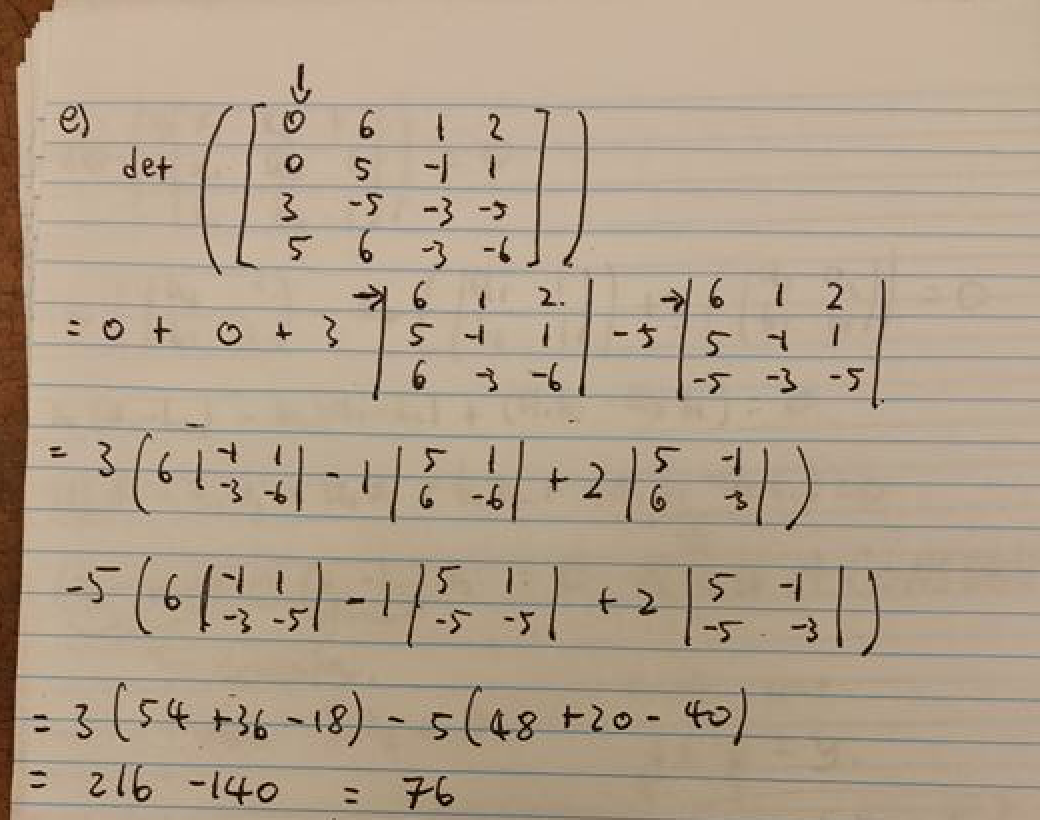
\includegraphics[scale=0.6]{determinant.png}
      	\caption{Determinant Calculation \label{fig:Determinant}}
\end{figure}
As you can see, cofactor expanding a 4x4 matrix ends up with 3x3 matrices which also needs to be calculated using cofactor expansion.
\textbf{Pro Tip: Pick a row/column with the most zeros in order to do the least amount of calculation.}

\subsection{Properties of Determinant}
\begin{enumerate}
\item It is possible perform cofactor expansion along any row or column. Suggested to do it along row or row with most zeros. 
\item If A is an nxn matrix that is Lower/Upper Triangular Matrix, them det(A) is the product of the diagonal entries. \\$det(A) = a_{11}a_{22}...a_{nn}$
\item If A is an nxn matrix, then det(A)=det$(A^T)$
\item Scalar Multiple of ith row or jth column scales the determinant\\
\begin{center}
$A = \begin{bmatrix}$
   $a_{11} & a_{12}\\ a_{21} & a_{22}$ 
 $\end{bmatrix}$
 $B = \begin{bmatrix}$
   $ta_{11} & ta_{12}\\ a_{21} & a_{22}$ 
 $\end{bmatrix}$\\
 det(B) = tdet(A)
 \end{center}
\item Swapping two rows or columns multiplies the determinant by -1
\begin{center}
$A = \begin{bmatrix}$
   $a_{11} & a_{12}\\ a_{21} & a_{22}$ 
 $\end{bmatrix}$
 $B = \begin{bmatrix}$
   $a_{21} & a_{22}\\ a_{11} & a_{12}$ 
 $\end{bmatrix}$\\
 det(B) = -det(A)
 \end{center}
 Every time a swapping happens, multiply the determinant by -1.
 \item Adding a scalar multiple of one row/column to another row
 \item If one row/column of an $n$x$n$ matrix contains only zeros, then det(A) = 0.\\
 This also means that if there is a row or column that repeats, then det(A) = 0 since row reduction does not change the determinant.
 
\end{enumerate}
Just as a clarification, even though we only learned EROs, column operations are valid while solving for determinants due to the property of det(A) = det($A^T$). 

\subsection{Cramer's Rule}
A system of linear equation can be represented as $A\vec{x}=\vec{b}$ where $A$ is the coefficient matrix, $\vec{x}$ is the vector for variables, and $\vec{b}$ is the vector made from ''answers''. Then, Cramer's Rule is defined as following:
\begin{center}
$x_i = detA_i/detA$
\end{center}
Where $A_i$ is A matrix but with $i$th column replaced with $\vec{b}$.
The advantage of Cramer's Rule is that it is possible to determine only one variable without solving for the whole system. Which means, if you only care about the value of one variable, you can reduce the amount of computation.\\
\textbf{ex}\\
Consider the system of equation \\
\begin{center}
$\begin{cases} 2x_1 - 7x_2 = 3 \\  5x_1+4x_2 = -17 \end{cases}$
\end{center}
The coefficient matrix will be $A = \begin{bmatrix}$
   $2 & -7\\ 5 & 4$ 
 $\end{bmatrix}$ and $\vec{b} = \begin{bmatrix}$
   $3\\ -17$ 
 $\end{bmatrix}$
It is important to note that if you are row reducing the A matrix and will continue to use that matrix, you must substitute in the \textbf{Row Reduced version of $\vec{b}$} or else you will yield incorrect answer. This is why I suggest only using row reduction to find the determinant, and use the original A matrix and $\vec{b}$.

\section{Eigenvector and Diagonalization}
The simplest description of Eigenvector and Eigenvalue is the following:\\
A vector that satisfies the condition \\
\begin{center}
$A\vec{v} = \lambda\vec{v}$
\end{center}
then $\vec{v}$ is the eigenvector and $\lambda$ are the eigenvalue of the respective eigenvector. The associated pair is called eigenpair.\\
In order to determine the eigenpairs, you must find the non-trivial solution to the above equation.
Mathematically, that is described as:
\begin{equation}
C(\lambda) = det(A-\lambda I) = \vec{0}
\end{equation}
I know you are not supposed to have two equal signs in a equation, but what that means is that the \textbf{Characteristic Polynomial, C($\lambda$)} is equal to the equation $det(A-\lambda I) = \vec{0}$. The determinant has to be zero since the unique solution is the trivial solution, or the zero vector. However, we want to find the \textbf{non-zero vector}, therefore we \textbf{do not} want the unique solution. This means that the determinant of the system is equal to zero.\
The hardest part of these eigenvalue question is factoring out the determinants so that you can easily find the roots. You might want to review how to do long division using polynomials in case you get stuck. Usually, if you row reduce properly \textbf{after} subtracting the $\lambda$, then you usually get nice polynomials to work with. However, if you do get stuck with higher order polynomial, knowing long division may be useful.\\
\textbf{It is important to note that you should not row reduce the matrix then subtract the $\lambda$. This will get you a different answers. You can row reduce after subtracting $\lambda$ to make the determinant calculation a bit easier.}\\
To find the eigenvectors associated with each eigenvalues, all you have to do is to find the general solution of the system \\
\begin{equation}
(A-\lambda I)\vec{v}= \vec{0}
\end{equation}
Note that since we already set our determinant of the system as 0, the resulting solution will have parameters. The eigenspace is described by the eigenvectors of the resulting matrix.\\

\subsection{Algebraic and Geometric Multiplicity}
When solving the characteristic polynomial, there are times when the same root (the eigenvalues) appear more than once. For example, if there is an equation such as 
\begin{center}
$0 = (\lambda -1)^2(\lambda +5)$
\end{center}
Then, the ''solutions'' to this equation are $\lambda = 1, \lambda = -5$. However, since the equation is $(\lambda -1)^2$, $\lambda = 1$ technically appears twice, but $\lambda = 5$ only appears once. 
The number of time each eigenvalue appears as the solution is called \textbf{Algebraic Multiplicity (AM)}.
After eigenvalues are calculated, the eigenvectors can be found by solving the system $(A-\lambda I)\vec{v}= \vec{0}$ like mentioned before. For example, given that:

\begin{center}
$A = \begin{bmatrix}$
   $2 & 2 & -6\\ 0 & 1 & 0\\0 & 0 & 1$ 
 $\end{bmatrix}$,
 $\lambda = 1$,\\
 then $A-\lambda I = \begin{bmatrix}$
   $1 & 2 & -6\\ 0 & 0 & 0\\0 & 0 & 0$ 
 $\end{bmatrix}$
\end{center}
The general solution to the system is 
\begin{center}
$\vec{v} = \begin{bmatrix}v_1 \\ v_2 \\ v_3 \end{bmatrix} = t \begin{bmatrix}-2 \\ 1 \\ 0 \end{bmatrix} + s  \begin{bmatrix}6 \\ 0 \\ 1 \end{bmatrix}$
where $s = v_2, t=v_3$
\end{center}
There are two eigenvectors, describing eigenspace of $\R^2$. The number of eigenvectors associated with eigenvalue, or the dimension of the eigenspace described by the eigenvectors is called the \textbf{Geometric Multiplicity (GM)}.
There is a theorem that compares AM and GM.
\begin{equation}
1 \leq Geometric Multiplicity \leq Algebraic Multiplicity
\end{equation}
This theorem tells us that GM cannot be greater than AM, and that they always have to be at least 1. This theorem comes in useful later when diagonalization is introduced. 

\subsection{Diagonalization}
The highlight of Diagonalization chaper is the following mathematical equation:
\begin{equation}
P^{-1}AP=D 
\end{equation}
A is the original matrix that we are trying to diagonalize.\\
Let eigenvectors of A be ${\vec{v_1}...\vec{v_n}}$ and their respective eigenvalues be ${\lambda_1...\lambda{n}}$
Then, P is the matrix formed by compiling the eigenvectors, $P = [\vec{v_1}...\vec{v_n}]$ and\\
$D = diag(\lambda_1...\lambda_n)$.\\
P and D does not have to compiled in order, but \textbf{the positions of the eigenvectors and eigenvalues must match}.\\
If the following equation is satisfied:
\begin{equation}
P^{-1}AP=B 
\end{equation}
Then it is said that matrix A and B are \textbf{Similar Matrices}.

If A and B are similar $n$ x $n$ matrices, then A and B have
\begin{enumerate}
\item The same determinant
\item The same eigenvalues 
\item The same rank
\item The same trace (The sum of diagonal entries)
\end{enumerate} \cite{Textbook}
\noindent 
Since the diagonal matrix also follows the same relationship as the similar matrices, A and diagonal matrix D also has the same properties of similar matrices. Diagonal matrices are advantageous in calculating the determinant and rank since only diagonal terms exist in D matrix.

\subsection{Diagonalization Theorem}\
Not all matrices are diagonalizable, and there are few theorems that tell us whether a matrix is diagonalizable. \\
Although there is a very explicit and general theorem,\\
\begin{center}
\noindent
An nxn matrix A can be diagonalized IFF there exists a basis for $\R^n$ of eigenvectors of A. 
If such basis ${\vec{v_1}...\vec{v_n}}$ exists, the matrix $P = [\vec{v_1}...\vec{v_n}]$ diagonalizes A to a diagonal matrix $D = diag(\lambda_1,...,\lambda{n})$, where $\lambda_i$ is an eigenvalue of A corresponding to $\vec{v_i}$ for $1\leq i \leq n$\\
\end{center}
\noindent
However, for the purposes digesting the theorem, the core of the above theorem is the following:\\
\begin{center}
\textbf{A matrix is diagonalizable if and only if every eigenvalue of a matrix A has its Geometric Multiplicity equal to its Algebraic Multiplicity}
\end{center}
\noindent
and from the above statement, we also know that:\\
\begin{center}
\textbf{If an $n$ x $n$ matrix has $n$ distinct eigenvalues, then A is diagonalizable}
\end{center}
\noindent
This is where the theorem mentioned above that shows the relationship between the number of AM and GM.\\
We know that if eigenvalue has 1 AM, then we know we do not need to check GM to know that it is 1. However, if an eigenvalue has more than 1 as its AM, then the ''diagonalizability'' (apparently this is not a word) is not guaranteed.  Therefore, if the question asks to see if matrix is diagonalizable and find the diagonal matrix, then it is better to find the eigenvectors of eigenvalues with AM $>$ 1 as it can \textbf{potentially save you time.}

\section{Complex Numbers}
Complex number is a new domain of numbers that are very useful in the future for some students.\\
Complex number has two forms: Rectangular and Polar Form. Each form has their advantages and both concepts will have to be learned for the exam.\\

\subsection{Rectangular Form}
Rectangular form of Complex Number is denoted as following:\\
\begin{equation}
z = x+yi
\end{equation}
where $x,y\in \R$, and $i^2 = -1$, or simply speaking, $\sqrt{-1} = i$.\\
$z = 0$ if and only if $x = 0$ \textbf{and} $y = 0$.\\
If $x = 0$, then z is \textbf{purely imaginary}, and if $y = 0$, then z is \textbf{purely real}.\\
This also gives us the conclusion that all real numbers are under the entity of complex numbers. \\
Some Definitions: Given that $z_1 = x_1 + y_1i$ and $z_2 = x_2+y_2i$
\begin{enumerate}
\item $z_1 = z_2$ if and only if $x_1 = x_2$ \textbf{and} $y_1 = y_2$
\item $z_1 + z_2 = (x_1 +  x_2) + (y_1+y_2)i$ or $(Re(z_1) + Re(z_2)) + (Im(z_1)+Im(z_2))i$
\item $tz_1 = t(x_1+y_1i) = tx_1 + ty_1i$
\item $z_1z_2 = (x_1+y_1i)(x_2+y_2i)=(x_1x_2-y_1y_2) + (x_1y_2+x_2y_1)i$ (Using FOIL)
\end{enumerate} \cite{Textbook}

\subsubsection{Complex Conjugate}
Given $z=x+yi$, the complex conjugate is defined as 

\begin{equation}
\overline{z} = x-yi
\end{equation}

As observed, the complex conjugate simply takes the negative of the imaginary portion of $z$. It is important to understand that conjugate can only taken when it is in rectangular form.  This is useful since 
\begin{equation}
\overline{z}z = x^2 + y^2
\end{equation}
This is same as the difference of square property $(x+y)(x-y) = x^2 + y^2$. Notice that multiplying complex number with itself results in purely real number. This is used to perform division of complex numbers in rectangular form with this formula.\\

\begin{equation}
\frac{z_1}{z_2} = \frac{z_1\overline{z_2}}{z_2\overline{z_2}}
\end{equation}
The complex conjugate of $z_2$ is multiplied both numerator and denominator since we want to get rid of the i term in the denominator. If there is $i$ term present in the denominator, then we cannot express it as proper rectangular form.

\subsubsection{Some Properties}
Here are some properties of complex numbers that may be useful in solving questions.\\
\begin{enumerate}
\item $\overline{\overline{z}} = z$ 
\item Purely Real iff $\overline{z} = z$
\item Purely Imaginary iff $\overline{z} = -z$
\item $\overline{z_1+z_2} = \overline{z_1} + \overline{z_2}$
\item $\overline{z_1z_2} = \overline{z_1}\:\overline{z_2}$
\item $\overline{(z)^n} = \overline{(z)}^n$
\item $z + \overline{z} = 2Re(z)$
\item $z - \overline{z} = 2iIm(z)$
\item $\overline{z}z = x^2 + y^2$
\end{enumerate} \cite{Textbook}

\subsection{Roots of Polynomial Equation}
Theorem: For $P(x) =a_nx^n + ... + a_nx^1+a_0$, if $z$ is a root of $P(x)$ then $\overline{z}$ is also a root of $P(x)$.\\
ex: $x^3 + 1= (x+1)(x^2-x+1)$ \\
The first root is $x = -1 + 0i$ and its conjugate is $\overline{x} = -1 -0i$, which are both the roots since they are the same number.\\
The second root, after using the quadratic formula, are\\
$z = \frac{1+\sqrt{3}i}{2}$, $\overline{z} = \frac{1-\sqrt{3}i}{2}$.\\

\subsection{Complex Plane}
Since complex numbers are written as $x+yi$, we can interpret complex number as a set of numbers $(x,y)$ similar to a set of points in space. This is why we can geometrically interpret complex number as a point in space/vector in space.\\
For $z = x+yi$, the set of point is $(x,y)$\\
\begin{figure}[!htb]
      	\centering
      	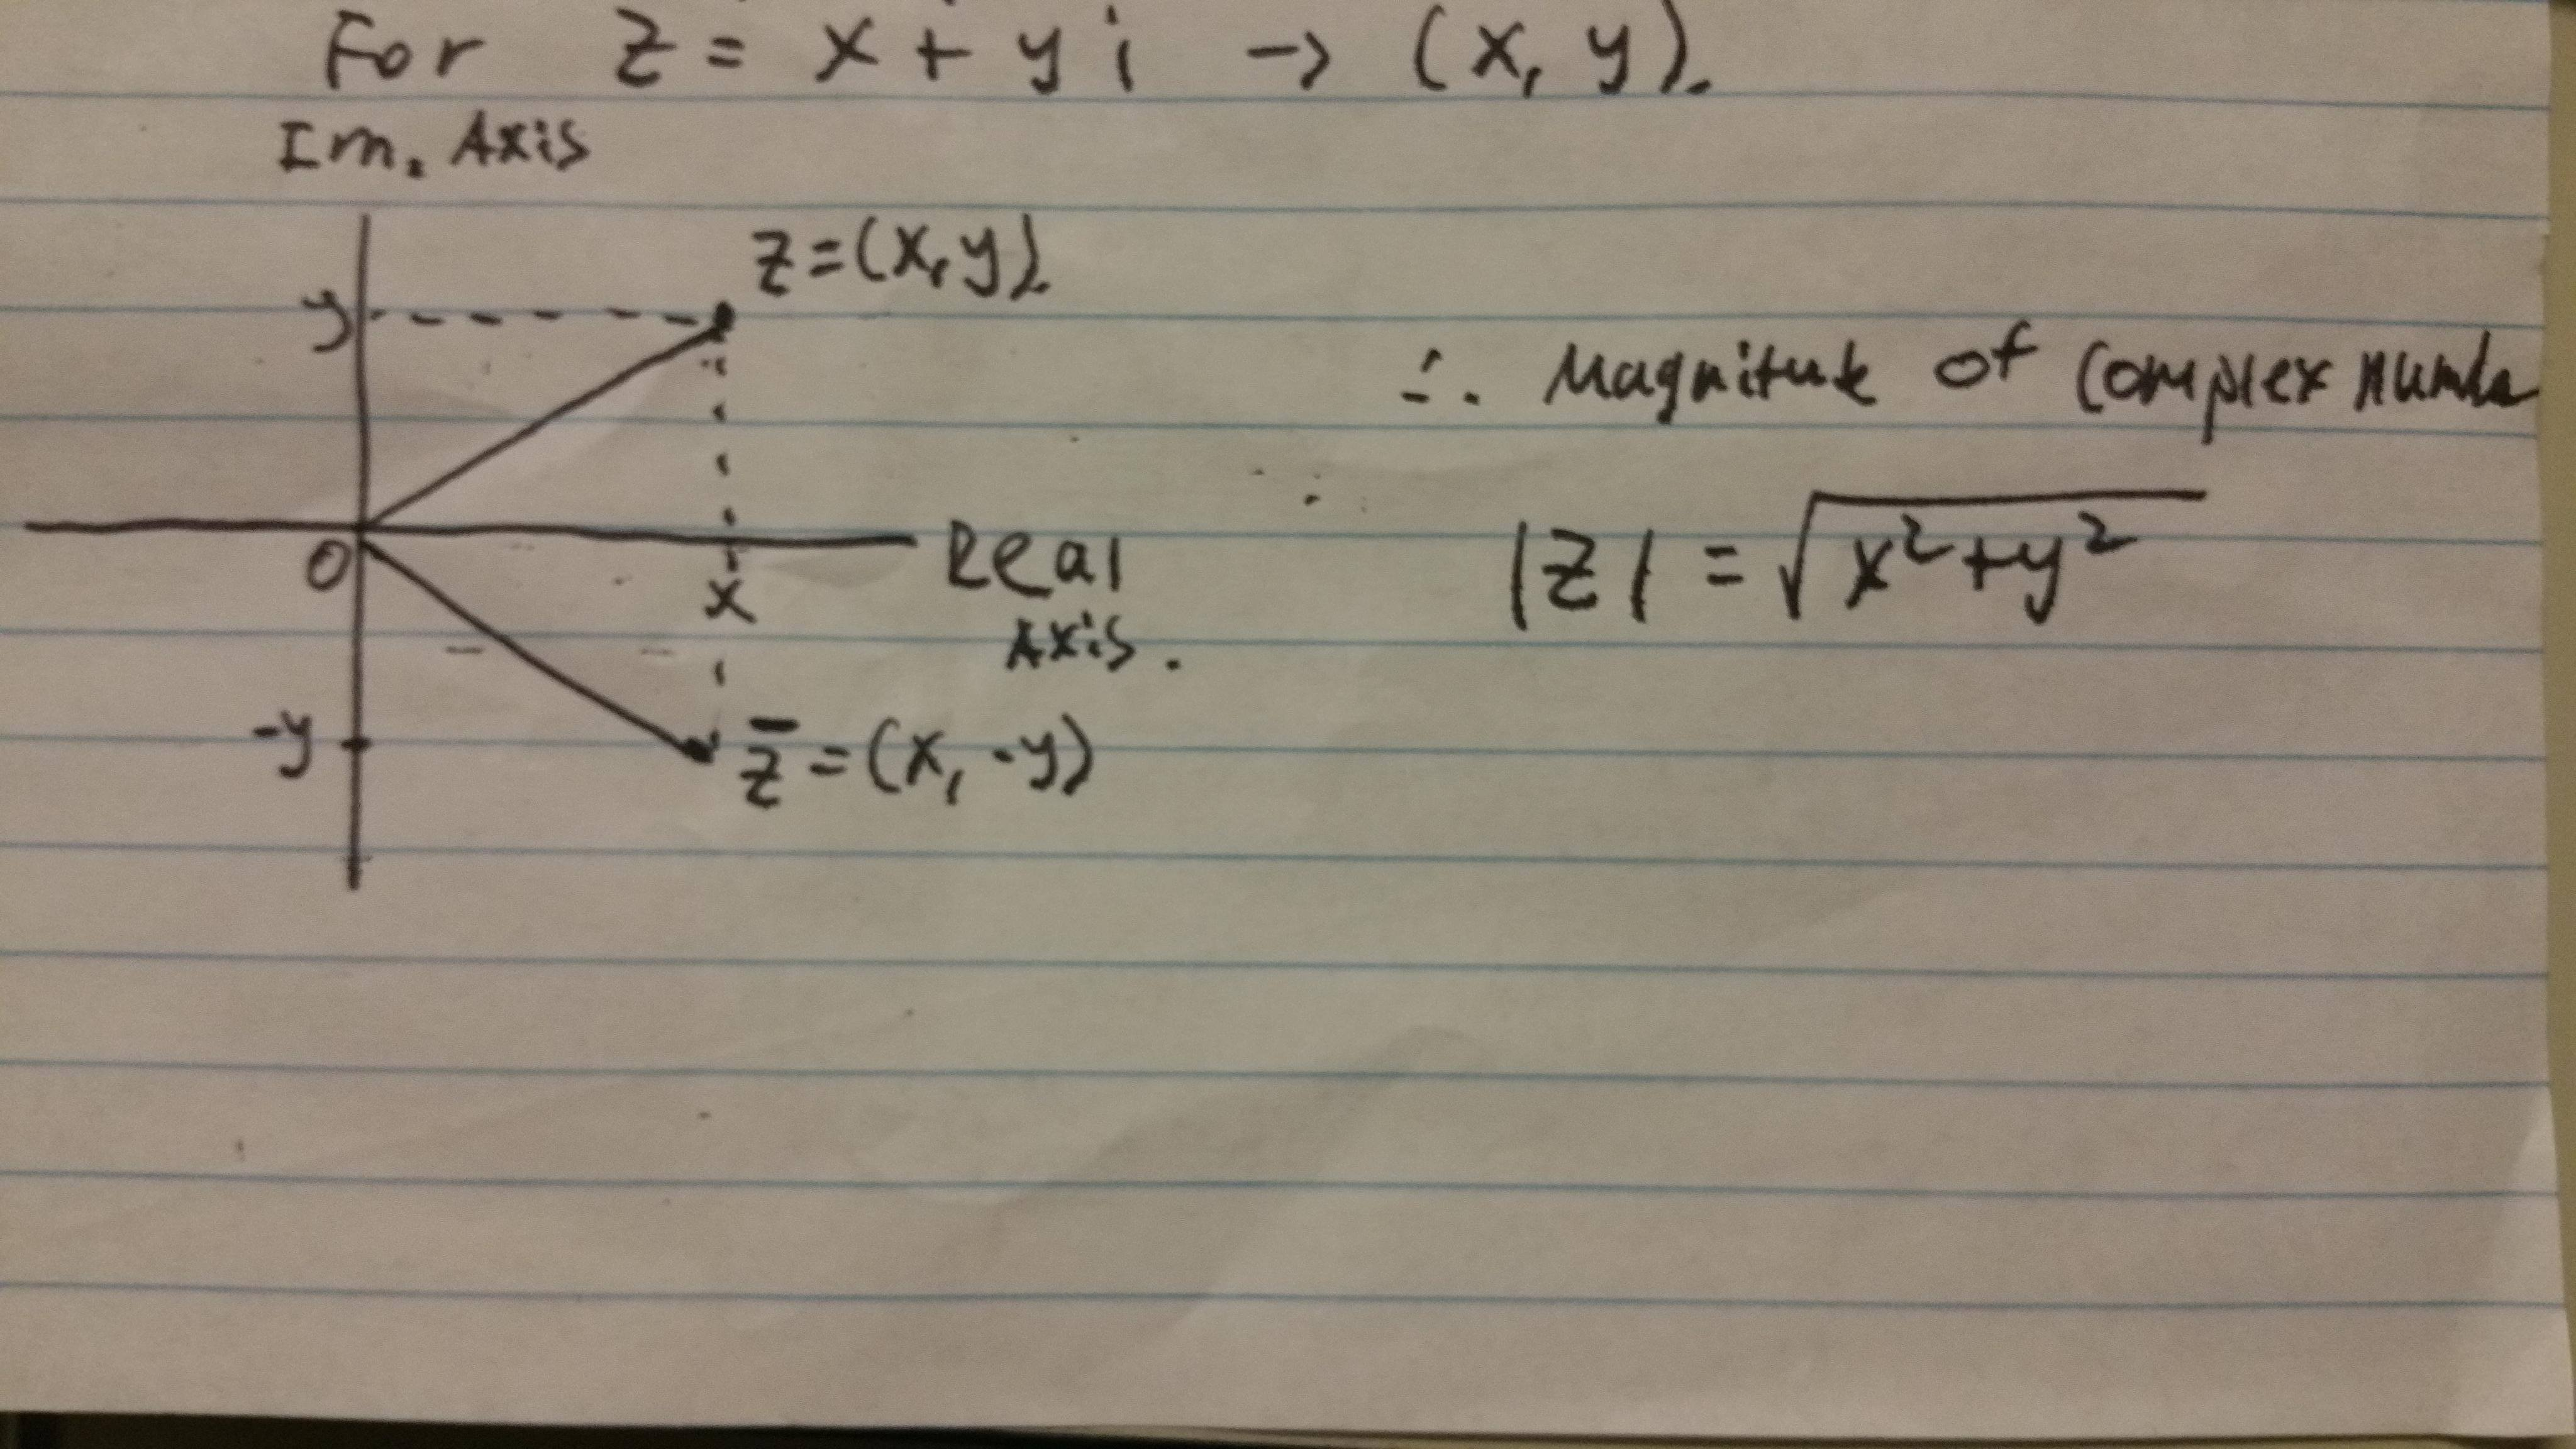
\includegraphics[scale=0.1]{ComplexPlane.jpg}
      	\caption{Complex Plane Diagram \label{fig:ComplexPlane}}
\end{figure}

\subsection{Polar Form}
Using $xy$ coordinate system is only one method of representing a position in space. Another method of representing a position in space is to represent it as magnitude of the vector and the amount of angle that it is displaced from a reference point (usually positive x axis). So instead of having $(x,y)$, it would be $(r,\theta)$.\\
The magnitude of the vector is determined by finding the length of the vector. Pythagorean Theorem can be used.\\
\begin{equation}
r = |z| = \sqrt{x^2+y^2}
\end{equation}
\begin{centering}
and 
\end{centering}
\begin{equation}
\begin{split}
x &= rcos\theta\\
y &= rsin\theta
\end{split}
\end{equation}
and $\theta$ can be found by solving two equations 
\begin{equation}
\begin{split}
\frac{x}{r} &= cos\theta\\
\frac{y}{r} &= sin\theta
\end{split}
\end{equation}
Note that you need to use both equations in order to \textbf{obtain full marks}, since this is the method that was presented in the textbook. However, you can simply use $\theta = arctan(\frac{x}{y})$ and use C.A.S.T. Rule to find out which quadrant the angle will reside in.

\begin{figure}[!htb]
      	\centering
      	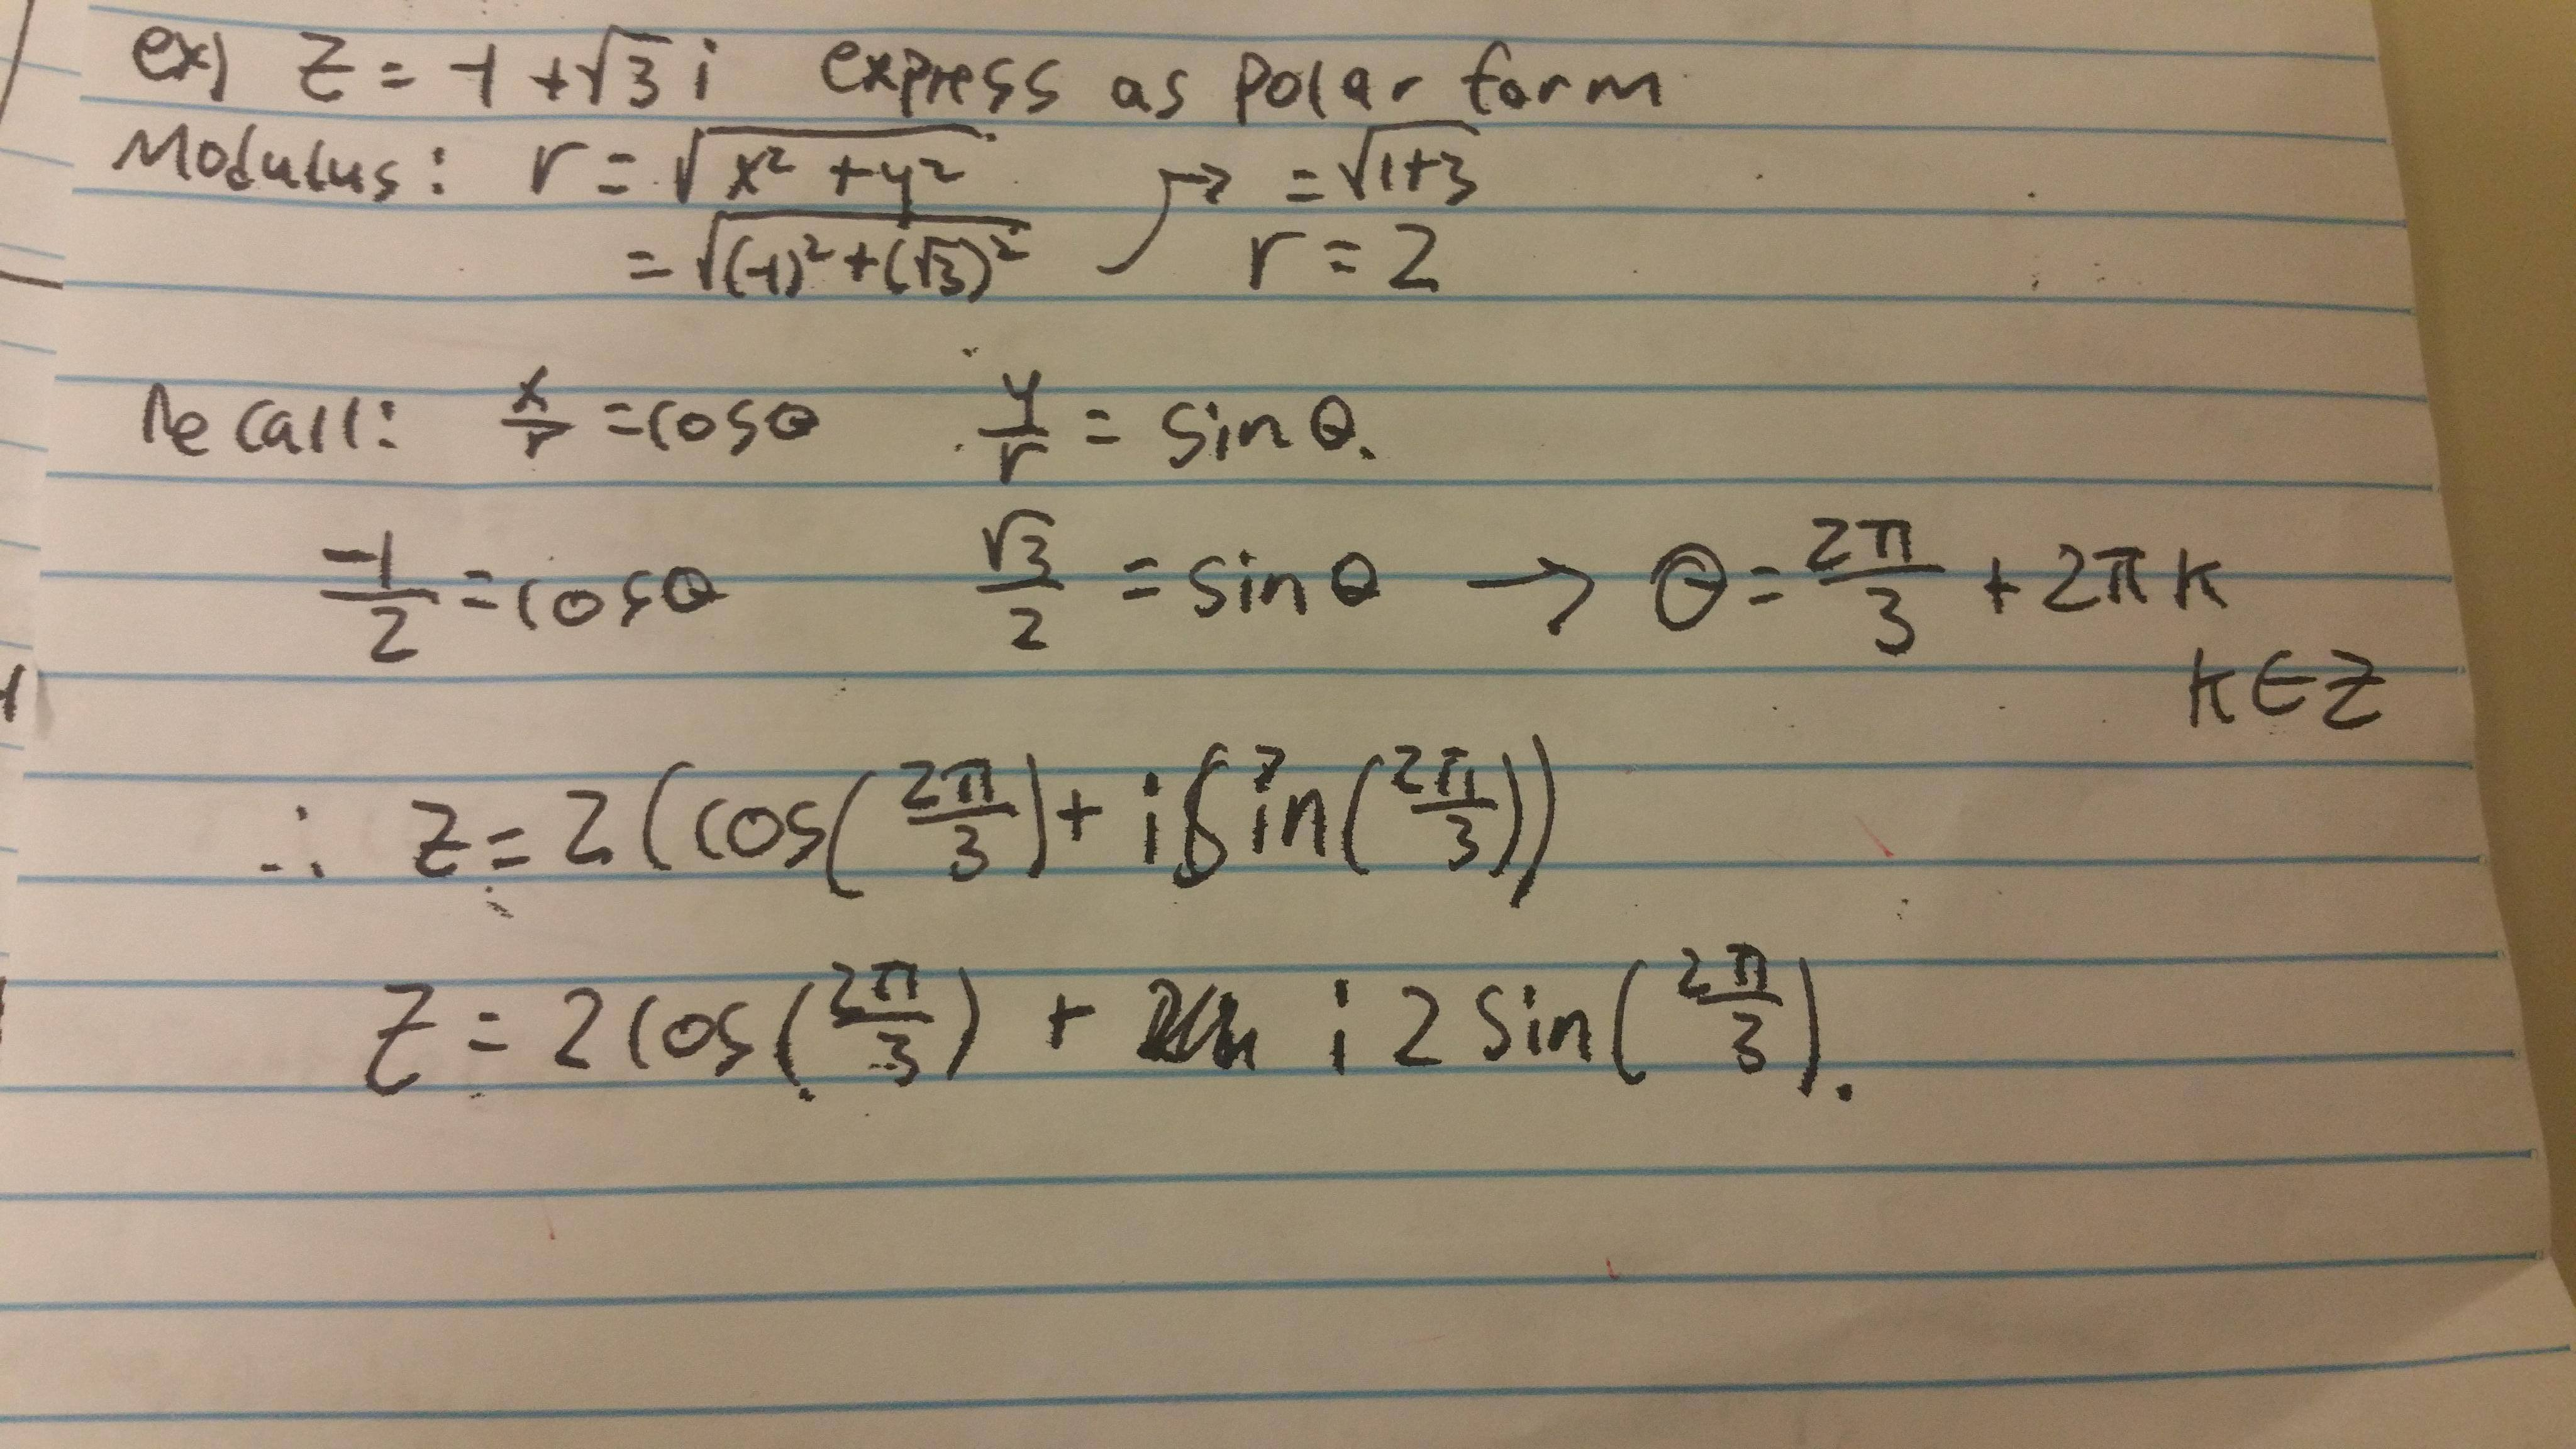
\includegraphics[scale=0.1]{PolarEx.jpg}
      	\caption{Example of Rectangular to Polar \label{fig:PolarEx}}
\end{figure}

\subsubsection{Multiplication and Division with Polar Form}
Multiplication and Division is actually a lot easier using polar coordinate. Recall the identity
\begin{equation}
\begin{split}
cos(\theta_1+\theta_2) &= cos\theta_1cos\theta_2 - sin\theta_1sin\theta_2\\
sin(\theta_1+\theta_2) &= sin\theta_1cos\theta_2 + cos\theta_1sin\theta_2
\end{split}
\end{equation}

From this, we can derive the two formulas
\begin{equation}
\begin{split}
z_1z_2 = r_1r_2(cos(\theta_1+\theta_2) + i(sin(\theta_1+\theta_2)))\\
\frac{z_1}{z_2} = \frac{r_1}{r_2}(cos(\theta_1-\theta_2) + i(sin(\theta_1-\theta_2)))
\end{split}
\end{equation}

and we can find that 
\begin{equation}
z^{-1} = \frac{1}{r}(cos(-\theta) + isin(-\theta))
\end{equation}

From the multiplication formula, we also can find another formula (also known as de Moivre's Formula)
\begin{equation}
z^n = r^n(cos(n\theta) + isin(n\theta))
\end{equation}
If power of a complex number in its rectangular form must be calculated, I suggest converting it to polar form, calculate the power, and converting it back if the power is \textbf{greater than 3}.

Therefore, we can conclude that:\\
\begin{center}
Addition/Subtraction is easier on Rectangular Form\\
Multiplication/Division is easier on Polar Form
\end{center}

\subsection{Euler's Formula}
One of the greatest mathematicians in the history of the world has created the relationship as following:
\begin{equation}
e^{i\theta} = cos\theta + isin\theta
\end{equation}
(Note, Euler is pronounced Oil-er \textbf{NOT} You-ler)\\

This means that polar form can also be represented as 
\begin{equation}
z = re^{i\theta}
\end{equation}


\subsection{$n^{th}$ Roots}
Recall that 
\begin{equation}
\begin{split}
z^n &= r^n(cosn\theta + isinn\theta) = r^ne^{ni\theta}
\end{split}
\end{equation}

In  order to find the nth root we observe that
\begin{equation}
\begin{split}
w^n &= z\\
w &= z^{\frac{1}{n}} 
\end{split}
\end{equation}

Therefore, we get the formula of $n^{th}$ root is 

\begin{equation}
w_k = r^{\frac{1}{n}}e^{\frac{i(\theta+2\pi k)}{n}}, k = 0,1...n-1
\end{equation}
(This equation was obtained by applying de Moivre's theorem from the last line of previous equation).
Until now, you only knew about the real roots. However, since $i^2 = -1$, it is possible to find the complex roots of numbers, and the real root is only a partial root of the system.

$k$ does not go until $n$, since after $n-1$, the roots actually start to repeat itself. \\
For example, let's find the 3rd root of $z = 1 + 0i$. $r = 1, \theta = 0, n=3$ are the knowns that we are calculated/given.\\
\textbf{1st Root}\\
$w_0 = r^{\frac{1}{n}}e^{i(\theta+2\pi k)/n} = 1^{\frac{1}{3}}e^{i(0+0)/3} = 1^{\frac{1}{3}} = 1$\\
\textbf{2nd Root}\\
$w_1 = r^{\frac{1}{n}}e^{i(\theta+2\pi k)/n} = 1^{\frac{1}{3}}e^{i(0+2\pi)/3} = 1^{\frac{1}{3}}e^{i2\pi/3}$\\
\textbf{3rd Root}\\
$w_2 = r^{\frac{1}{n}}e^{i(\theta+2\pi k)/n} = 1^{\frac{1}{3}}e^{i(0+4\pi)/3} = 1^{\frac{1}{3}}e^{i4\pi/3}$\\
\textbf{4th Root}\\
$w_4 = r^{\frac{1}{n}}e^{i(\theta+2\pi k)/n} = 1^{\frac{1}{3}}e^{i(0+6\pi)/3} = 1^{\frac{1}{3}}e^{i6\pi/3} = 1$\\
Notice how after $(n-1)$ term, the roots are going to repeat itself.\\
$n^{th}$ root questions are very straight forward, as you just need to use the formula that is derived from de Moivre's theorem.

Another example:
\begin{align*}
5i &= 5e^{i(\frac{\pi}{2})} \\
R &= 5 \\
\theta &= \frac{\pi}{2}
\end{align*}

At $k=0$, 
\begin{align*}
w_0 &= 5^{\frac{1}{3}} e^{i(\frac{(\frac{\pi}{2})}{3})} \\
&= 5^{\frac{1}{3}} e^{i(\frac{\pi}{6})} 
\end{align*}

At $k=1$, 
\begin{align*}
w_1 &= 5^{\frac{1}{3}} e^{i(\frac{\frac{\pi}{2} + 2\pi}{3})} \\
&= 5^{\frac{1}{3}} e^{i(\frac{5\pi}{6})} 
\end{align*}

At $k=2$, 
\begin{align*}
w_2 &= 5^{\frac{1}{3}} e^{i(\frac{\frac{\pi}{2} + 4\pi}{3})} \\
&= 5^{\frac{1}{3}} e^{i(\frac{9\pi}{6})} 
\end{align*}

\section{Vector Spaces}
Vector space is any space that satisfies the 10 axioms that are found in your textbook (you know which one I am talking about). Luckily, as for final exam in Fall 2017, you do not need to memorize nor need to prove whether a space is a vector space or not. 
Until now, we were only dealing with \textbf{vectors}, but \textbf{polynomials}, and \textbf{matrices} are other types of vectorspaces that satisfies the 10 axioms. Some notations are following: \\\\
\begin{centering}
$\mathbf{P_n}$: Set of all polynomials of degree \textbf{AT MOST} $n$\\
$\mathbf{R^n}$: Set of all vectors in $n^{th}$ dimension\\
$\mathbf{M(m,n)}$: Set of all $m$x$n$ matrices \\
\end{centering}

\subsection{Subspaces}
Define subspace generally, suppose $V$ is a vector space, a non-empty subset  $U$ or $V$ is a subspace of $V$ if it follows the two properties:\\
\begin{centering}
\textbf{S1}: $x + y \in U, \; x,y \in U$\\
\textbf{S2}: $tx \in U, \;, x\in U, t\in\R$\\ 
\end{centering}
(Zero vector existing is technically proven if the other two are proven, but you should still prove that the zero vector exists initially).

\subsection{Homogeneous System of Linear Equation}
You may encounter a type of question worded as such:\\
\textbf{Find a homogeneous system of linear equations that defines this set.}\\
Here are two examples to help you understand how to solve these type of questions.
\\
\begin{equation}
\begin{split}
Span
\left\{\begin{bmatrix}
1 \\
0 \\
0 \\
\end{bmatrix},
\begin{bmatrix}
0 \\
1 \\
0 \\
\end{bmatrix}\right\}
\end{split}
\end{equation}
\\
\begin{equation}
\begin{split}
t_1\begin{bmatrix}
1 \\
0 \\
0 \\
\end{bmatrix}
+
t_2\begin{bmatrix}
0 \\
1 \\
0 \\
\end{bmatrix}
=
\begin{bmatrix}
x_1 \\
x_2 \\
x_3 \\
\end{bmatrix}
\end{split}
\end{equation}
\\
\begin{equation}
\begin{amatrix}{2}
1 & 0 & x_1 \\ 0 & 1 & x_2 \\ 0 & 0 & x_3
\end{amatrix}
\end{equation}\\
In order for this system to be consistent, $x_1 = t_1$ and $x_2 = t_2$ but $x_3 = 0$ is a MUST\\
$\therefore$ The homogeneous equation that defines this set is $x_3 = 0$\\
\\A3 e)\\
\begin{equation}
\begin{split}
Span
\left\{\begin{bmatrix}
1 \\
0 \\
1 \\
0 \\
\end{bmatrix},
\begin{bmatrix}
2 \\
-1 \\
1 \\
1 \\
\end{bmatrix}\right\}
\end{split}
\end{equation}
\begin{equation}
\begin{split}
\begin{amatrix}{2}
1 & 2 & x_1 \\ 0 & -1 & x_2 \\ 1 & 1 & x_3 \\ 0 & 1 & x_4
\end{amatrix}
\mathtt{\sim}
\begin{amatrix}{2}
1 & 2 & x_1 \\ 0 & -1 & x_2 \\ 0 & 0 & -x_1 - x_2 + x_3 \\ 0 & 0 & x_2 + x_4
\end{amatrix}
\end{split}
\end{equation}\\
\begin{equation}
Must \colon
\begin{cases}
-x_1 -x_2 + x_3 = 0\\
x_2 + x_4 = 0
\end{cases}
\end{equation}\\
These two homogenous equations define the set.

 
 
\newpage
\begin{appendices}
\appendix 
\section{Compilation of Useful Formulas}
\label{appendix:Formula}
\noindent
\textbf{Projection}: $\vectorproj[x]{y} = \frac{\vec{x}\cdot\vec{y}}{{||\vec{x}||}^2}\vec{x}$\\\\
\noindent
\textbf{Norm of Projection}: $||\vectorproj[x]{y}|| = |\frac{\vec{y}\cdot\vec{x}}{||\vec{x}||}|$\\\\
\noindent
\textbf{Perpendicular}: $\vectorperp[x]{y} = \vec{y} - \vectorproj[x]{y}$\\\\
\noindent
\textbf{Shortest Distance (Line)}: $||\vectorperp[d]{{PQ}}||$ where P is point on line, Q is point not on line, and d is direction vector of line.\\\\
\noindent
\textbf{Shortest Distance (Plane)}: $||\vectorproj[n]{{PQ}}||$ where P is point on Place, Q is point not on plane.\\\\
\noindent
\textbf{Closest Point to a Plane}: $\vec{OR} = \vec{OQ} + \vec{QR} = \vec{OQ} + \vectorproj[n]{QP}$ where P is point on plane, Q is point not on plane R is point that has to be found\\\\
\noindent
\textbf{Volume of Parallelepiped}: V = $|\vec{u}\cdot\vec{w}$x$\vec{v}|$
or V = $|det(\vec{u}\;\vec{w}\; \vec{v})|$ (This works for n-d parallelotrope)\\\\
\noindent
\textbf{Determinant of 2x2 Matrix}: det(A) = $a_{11}a_{21} - a_{21}a_{22}$\\\\
\noindent
\textbf{Determinant of nxn Matrix}: det(A) = $det(A) = a_{11}C_{11} + a_{12}C_{12}+...+a{1n}C_{1n}$ where $C_{ij} = (-1)^{i+j}detA(i,j)$\\\\
\noindent
\textbf{Eigenvalue}: $det(A-\lambda I) = 0$ The roots of this polynomial is the eigenvalues\\\\
\noindent
\textbf{Eigenvector}: General Solution to the system $A-\lambda I = \vec{0}$\\\\
\noindent
\textbf{Diagonal Matrix}: $P^{-1}AP = D$\\\\
\noindent
\textbf{Multiplication of Complex Number}: $z_1z_2 =(x_1x_2-y_1y_2) + (x_1y_2+x_2y_1)i, \; z_1z_2 = r_1r_2(cos(\theta_1+\theta_2) + i(sin(\theta_1+\theta_2)))$\\\\
\noindent
\textbf{Division of Complex Number}: $\frac{z_1}{z_2} = \frac{z_1\overline{z_2}}{z_2\overline{z_2}}, \; \frac{z_1}{z_2} = \frac{r_1}{r_2}(cos(\theta_1-\theta_2) + i(sin(\theta_1-\theta_2)))$\\\\
\textbf{$n^{th}$ Root of Complex Number}: $w_k = r^{\frac{1}{n}}e^{\frac{i(\theta+2\pi k)}{n}}, k = 0,1...n-1$\\\\
\noindent

\thispagestyle{empty}
\end{appendices}

\newpage
\begin{thebibliography}{1}
\bibitem{Textbook}
D. Norman and D. Wolczuk, An Introduction to Linear Algebra for Science and Engineering. Don Mills, Ont.: Addison Wesley, 2012.


\end {thebibliography}


 
\end{document}
